\section{Correlations between Metadata and Detection Rate}
\label{sec:corr}
In this section, we study factors influencing detection rate of PE submissions.
A higher detection indicates a more malicious of a submitted file viewed by anti-virus engines.  
Our study is conducted from 4 aspects: reputation of source id, submission history, 
file size, and source country.

\begin{figure*}[!htb]
\minipage{0.31\textwidth}
  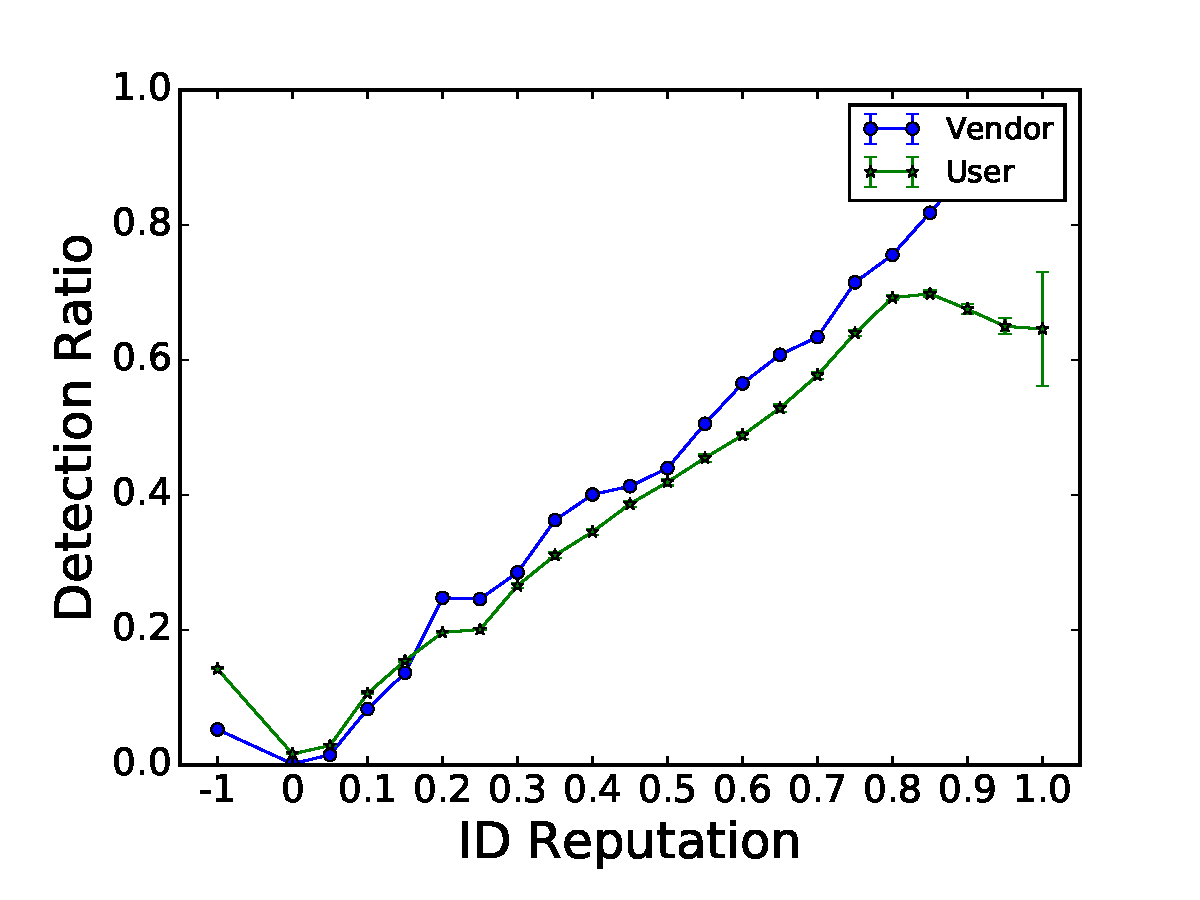
\includegraphics[width=\linewidth]{figure/IDReputation}
  \mycaption{fig:idreputation}{The relation between source id's previous reputation and detection rate.}
{\footnotesize{(How detection rate changes with the value of source id's reputation. Each reputation is rounded up to nearest 0.05.
Reputation -1 means the source id did not make any submission before. 95\% confidence interval is also drawn 
for each point.)}}
\endminipage\hfill
\minipage{0.31\textwidth}
  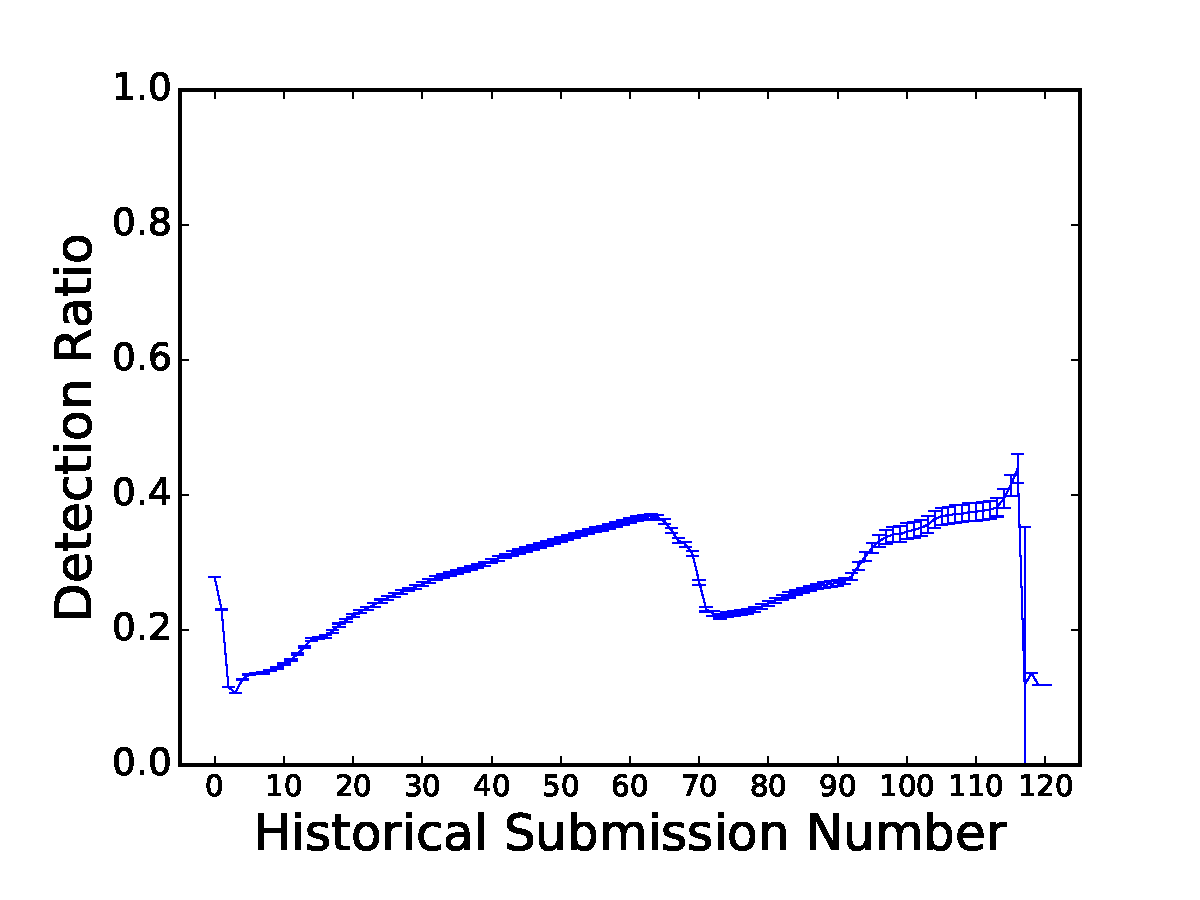
\includegraphics[width=\linewidth]{figure/SubNum}
  \mycaption{fig:hisnum}{The relation between historical submission number and detection rate.}
  {\footnotesize{(How detection rate changes with historical submission number. 
Each historical number is rounded up to nearest 5.
95\% confidence interval is also drawn for each point.)}}
\endminipage\hfill
\minipage{0.31\textwidth}%
  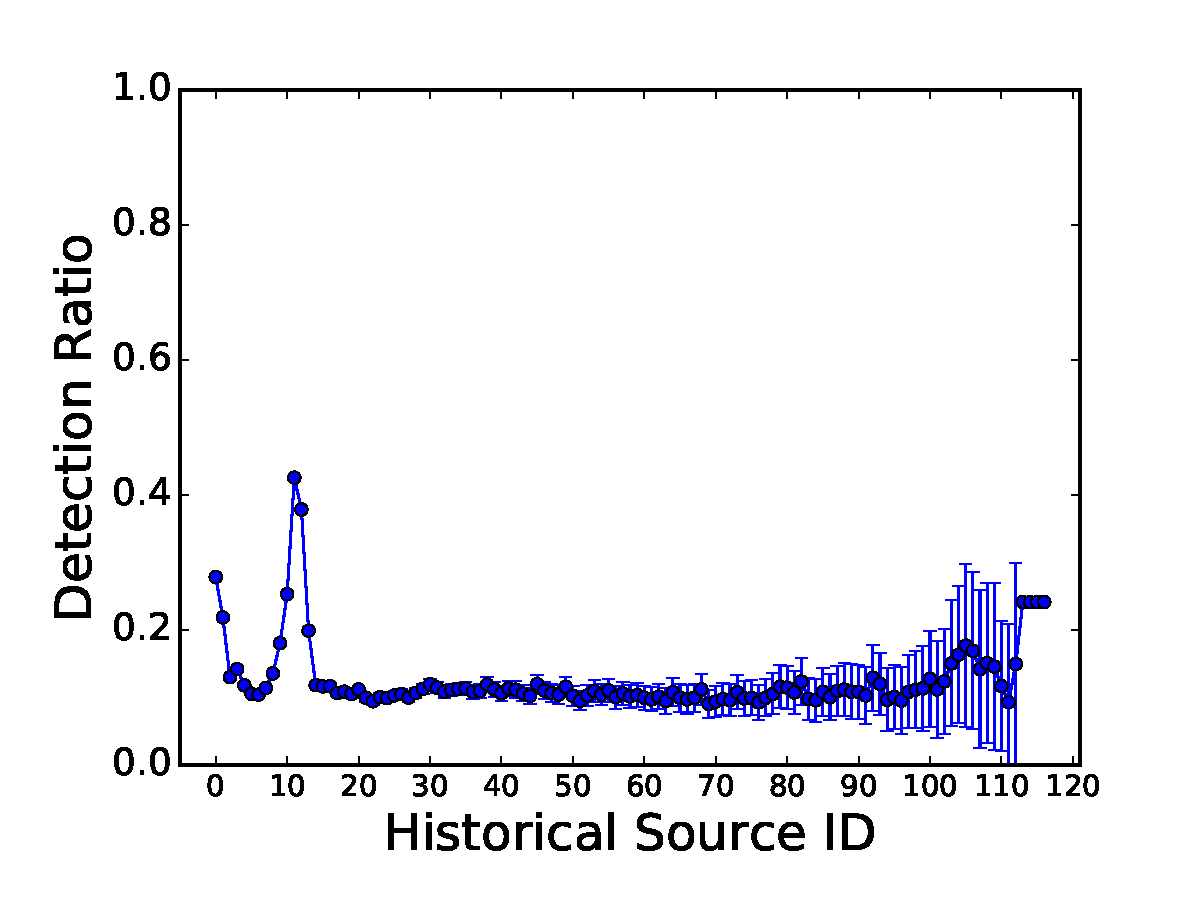
\includegraphics[width=\linewidth]{figure/SubID}
  \mycaption{fig:hisid}{The relation between the number of historical source ids and detection rate.}
{\footnotesize{(How detection rate changes with the number of historical source ids. 
Each historical number of source ids is rounded up to nearest 5.
95\% confidence interval is also drawn for each point.)}}
\endminipage\hfill

%\vspace{-0.2in}
\end{figure*}


\subsection{Reputation of Source ID}

\label{sec:reputation}

Previous work~\cite{GuoICSE2010} reported correlation between bug reporter’s reputation and the likelihood for the bug being fixed. 
We also observe correlation between the reputation of source id and submission’s detection rate. 

%\theoremstyle{definition}
\begin{definition}{Reputation:}
Given a submission $S$ with source id $I$, 
we define the reputation of $I$ when conducting the submission $S$ as the average detection rate for all submissions conducted by $I$ before $S$. 
If $I$ did not make any submission before, we define the reputation to be $-1$. 
\end{definition}

For around 14\% PE submissions, VirusTotal fails to provide source id information. 
We filter out these submissions, when computing reputation.
All other PE submissions are conducted by 613 thousand source ids. 
More than half source ids (66\%) only conduct submission once. 
We filter source ids conducting more than 1 million PE submissions in our data set, 
because we think these are anti-virus vendors routinely test their products. 

When calculating reputation, we sort all submissions from the same source id chronologically, 
and calculate reputation for each source id when conducting each submission. 
We round up each calculated reputation to nearest 0.05. 
We group submissions based on source ids' reputation when conducting submissions, 
and we plot average detection rate and 95\% confidence interval for each group in Figure~\ref{fig:idreputation}. 
Except the point with reputation 1, all other confidence intervals are invisible.  

As shown in Figure~\ref{fig:idreputation}, 
there is a rough increase for detection rate as the increase of source id's reputation, 
with the exception for the point with reputation -1 and the point with reputation 1. 
It is interesting to observe that first submissions conducted by different source ids have higher 
detection rate than submissions conducted by ids with reputation 0, 
and it is difficult for source ids with highest reputation to always submit files detected by all engines. 
Correlation between source id's reputation and detection rate indicates 
that it is feasible to use source ids' submission history to predict their future submissions.



\subsection{Submission History}
\label{sec:history}

\begin{figure*}[!htb]
\minipage{0.31\textwidth}
  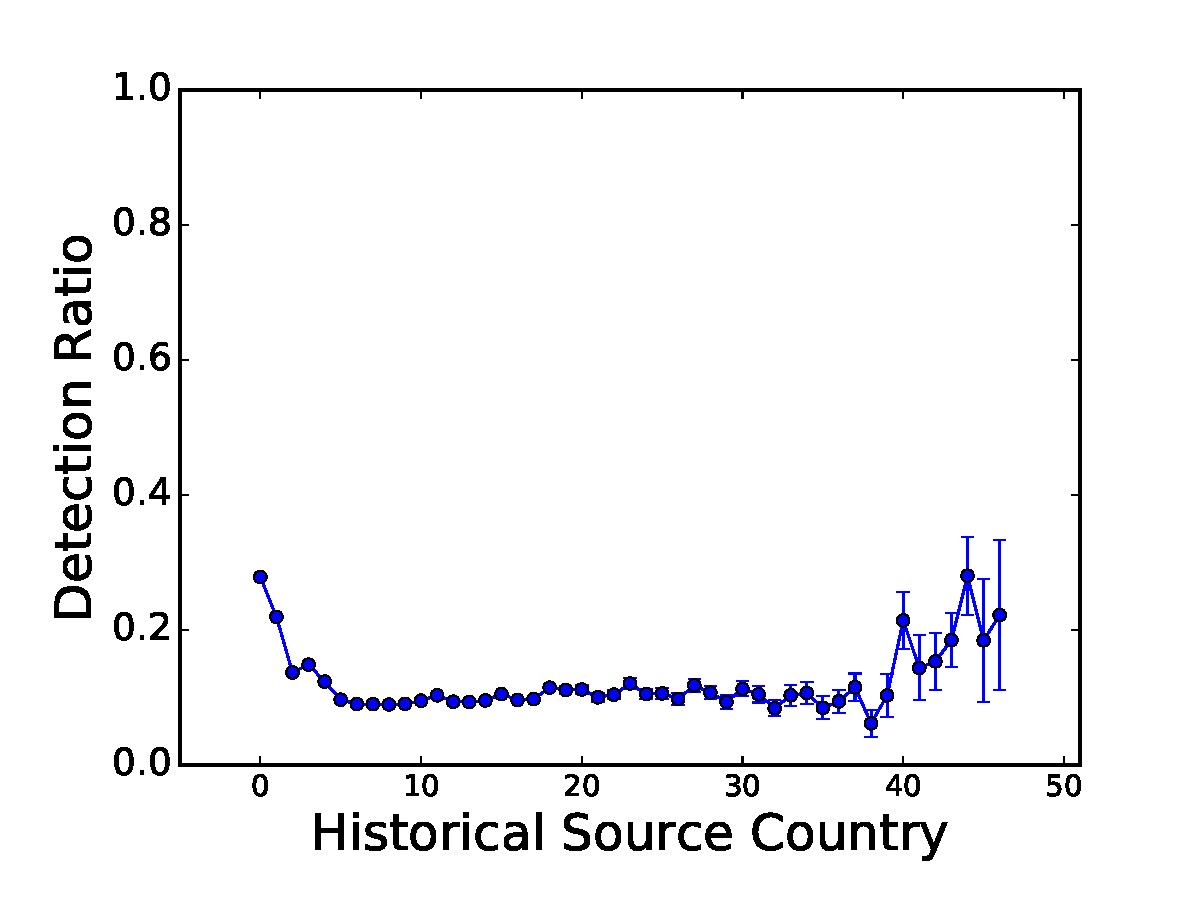
\includegraphics[width=\linewidth]{figure/SubCountry}
  \mycaption{fig:hiscountry}{The relation between the number of historical source countries and detection rate.}
{\footnotesize{(How detection rate changes with the number of historical source countries.
95\% confidence interval is also drawn for each point.)}}
\endminipage\hfill
\minipage{0.31\textwidth}
  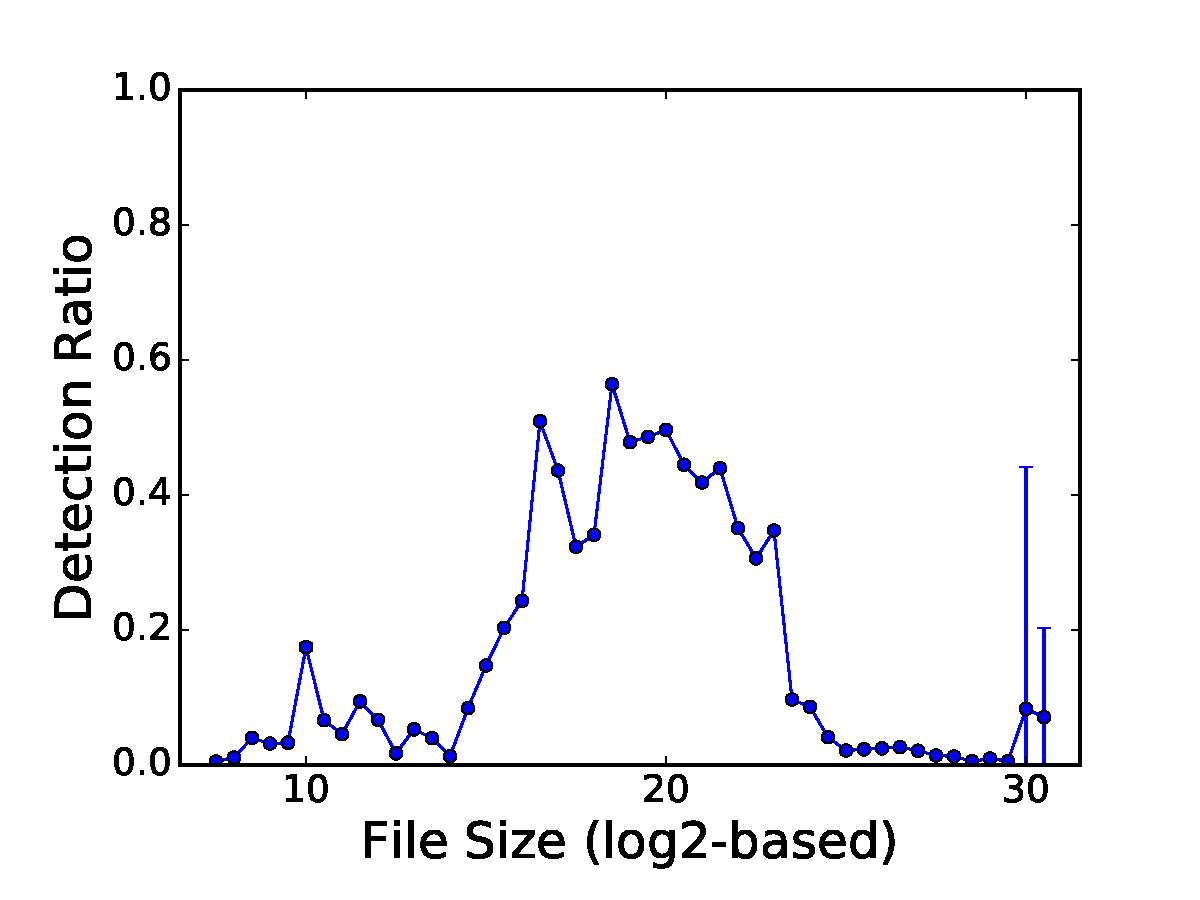
\includegraphics[width=\linewidth]{figure/size}
  \mycaption{fig:size}{How detection rate changes with file size.}
  {\footnotesize{(How detection rate changes with log2-based file size.
Results from log2 are rounded up to nearest 0.5.
95\% confidence interval is also drawn for each point.)}}
\endminipage\hfill
\minipage{0.31\textwidth}%
  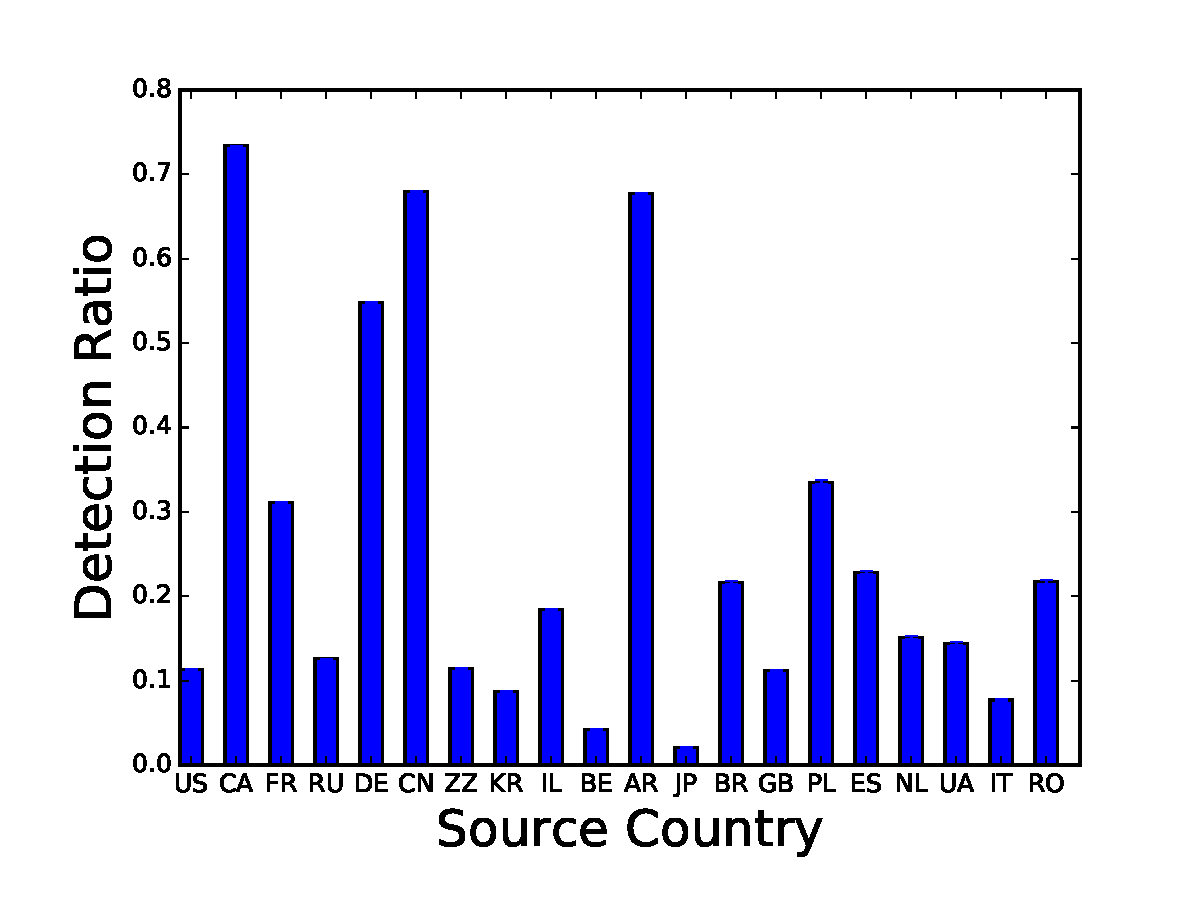
\includegraphics[width=\linewidth]{figure/Country}
  \mycaption{fig:Country}{Average detection rate for top 20 countries.}
{\footnotesize{(Average detection rate for submissions from countries ranking 
in top 20 in making PE submissions to VirusTotal. 
95\% confidence interval is also drawn for each country.)}}
  %\label{fig:aveUncover}
\endminipage\hfill

%\vspace{-0.2in}
\end{figure*}

One file could be submitted more than once to VirusTotal. 
Given a submission, we also study whether information for historical 
submissions of the same file influences detection rate for the current submission. 

{\textit{\underline{Historical submission number.}}}
We sort submissions for each file chronologically, 
and then calculate the correlation between detection rate and historical submission number for each submission. 
All historical submission numbers are rounded up to the nearest 5. 
How detection rate changes with historical submission number is shown in Figure~\ref{fig:hisnum}. 
The curve decreases from 0 to 10, increases from 10 to 65, decreases from 65 to 75, and increases after 75. 

We think there are two factors influencing whether detection rate would increase or decrease.
One is the percentage of benign files submitted to VirusTotal, 
and with more benign files submitted, detection rate will decrease.   
The other one is the percentage of engines identifying the submitted malwares, 
and with more engines identifying the malware, detection rate will increase. 
In the two stages of detection rate decreasing, 
VirusTotal users stop submitting identified malwares, 
and the increase of percentage of benign files submitted to VirusTotal dominates. 
In the the two stages of detection rate increasing, 
more engines can identify submitted malwares, 
and the increase of percentage of engines identifying submitted malwares dominates. 

{\textit{\underline{Historical source id.}}}
One file could be submitted by one source id multiple times, 
and could also submitted by different source ids. 
We study correlation between the number of historical source ids and detection rate. 
Each number of historical source ids is rounded up to nearest 5. 
Average detection rate and confidence interval for each number of historical source ids are shown in Figure~\ref{fig:hisid}. 
Confidence intervals are invisible before 80. 
Detection rate is higher for historical source ids less than 15, compared with historical source ids more than 15.
The number of historical source ids reflects the popularity of a submitted file.
Figure~\ref{fig:hisid} shows that when popularity of a file larger than a certain threshold, like 15 source ids, 
it is unrelated to detection rate and how malicious of the file viewed by anti-virus engines. 


{\textit{\underline{Historical source country.}}}
One file could also be submitted from different countries. 
The number of historical source countries also reflect the popularity of a submitted file. 
The correlation between detection rate and the number of historical source countries in 
Figure~\ref{fig:hiscountry} shows similar trend as the correlation between detection rate 
and the number of historical source ids in Figure~\ref{fig:hiscountry}. 

Figure~\ref{fig:hisnum}, Figure~\ref{fig:hisid}, and Figure~\ref{fig:hiscountry} show that 
when historical numbers fall into certain range, they are correlated with detection rate. 

\subsection{File Size}
\label{sec:size}

For each submission, we round up binary logarithm for its file size to nearest 0.5,
and calculate average detection rate for submissions with the same preprocessed file size.
Average detection rate and 95\% confidence interval for each preprocessed 
file size are shown in Figure~\ref{fig:size}.
Except for the last two points, all other confidence intervals are invisible.   
Files with size from 90KB to 4MB have average higher detection rate, which is more than 0.2. 

\subsection{Source Country}
\label{sec:country}

All PE submissions in our collection are conducted from 222 countries, 
and for roughly 17\% PE submissions, 
VirusTotal fails to provide their source country information. 
We rank source countries, based on their submission numbers. 
Average detection rate for top 20 source countries are calculated and shown in 
Figure~\ref{fig:Country}. 
Confidence intervals are also drawn for each source country, 
and all confidence intervals are almost invisible. 
From Figure~\ref{fig:Country}, 
we can see that submissions source countries are correlated with detection rate.

\subsection{Discussion}

{\textit{\underline{How to use our data?}}}
As we discussed from Section~\ref{sec:reputation} to Section~\ref{sec:country}, 
source ID reputation, historical number in certain range, file size, 
and source country are highly correlated with detection rate. 
Future work could train a regression model to combine all these factors together and 
predict how many engines could detect a malware or how malicious a malware is. 
By using the regression model or our studying results alone, 
security experts prioritize malwares, and focus their efforts on malwares which are more malicious. 
Anti-virus vendors could inspect results which are variant from our studying results 
to identify possible false positives or false negatives in their products. 

{\textit{\underline{Limitations of our study.}}}
As we discussed in Section~\ref{sec:meth}, our study is binded with our methodology.
We do not have any data before 05/07/2016, 
which may cause some reputation and historical numbers 
we calculate different from their real values. 
However, we think we can tolerate this error, 
since we conduct our study in a relatively long time range and in a large scale. 
In the future, we could design our reputation and historical metrics based on a tunable time windows, and investigate whether correlations still exist.   